
\section{\biochem}
\label{sec:juliaball}


\begin{figure*}[t]
	\centerline{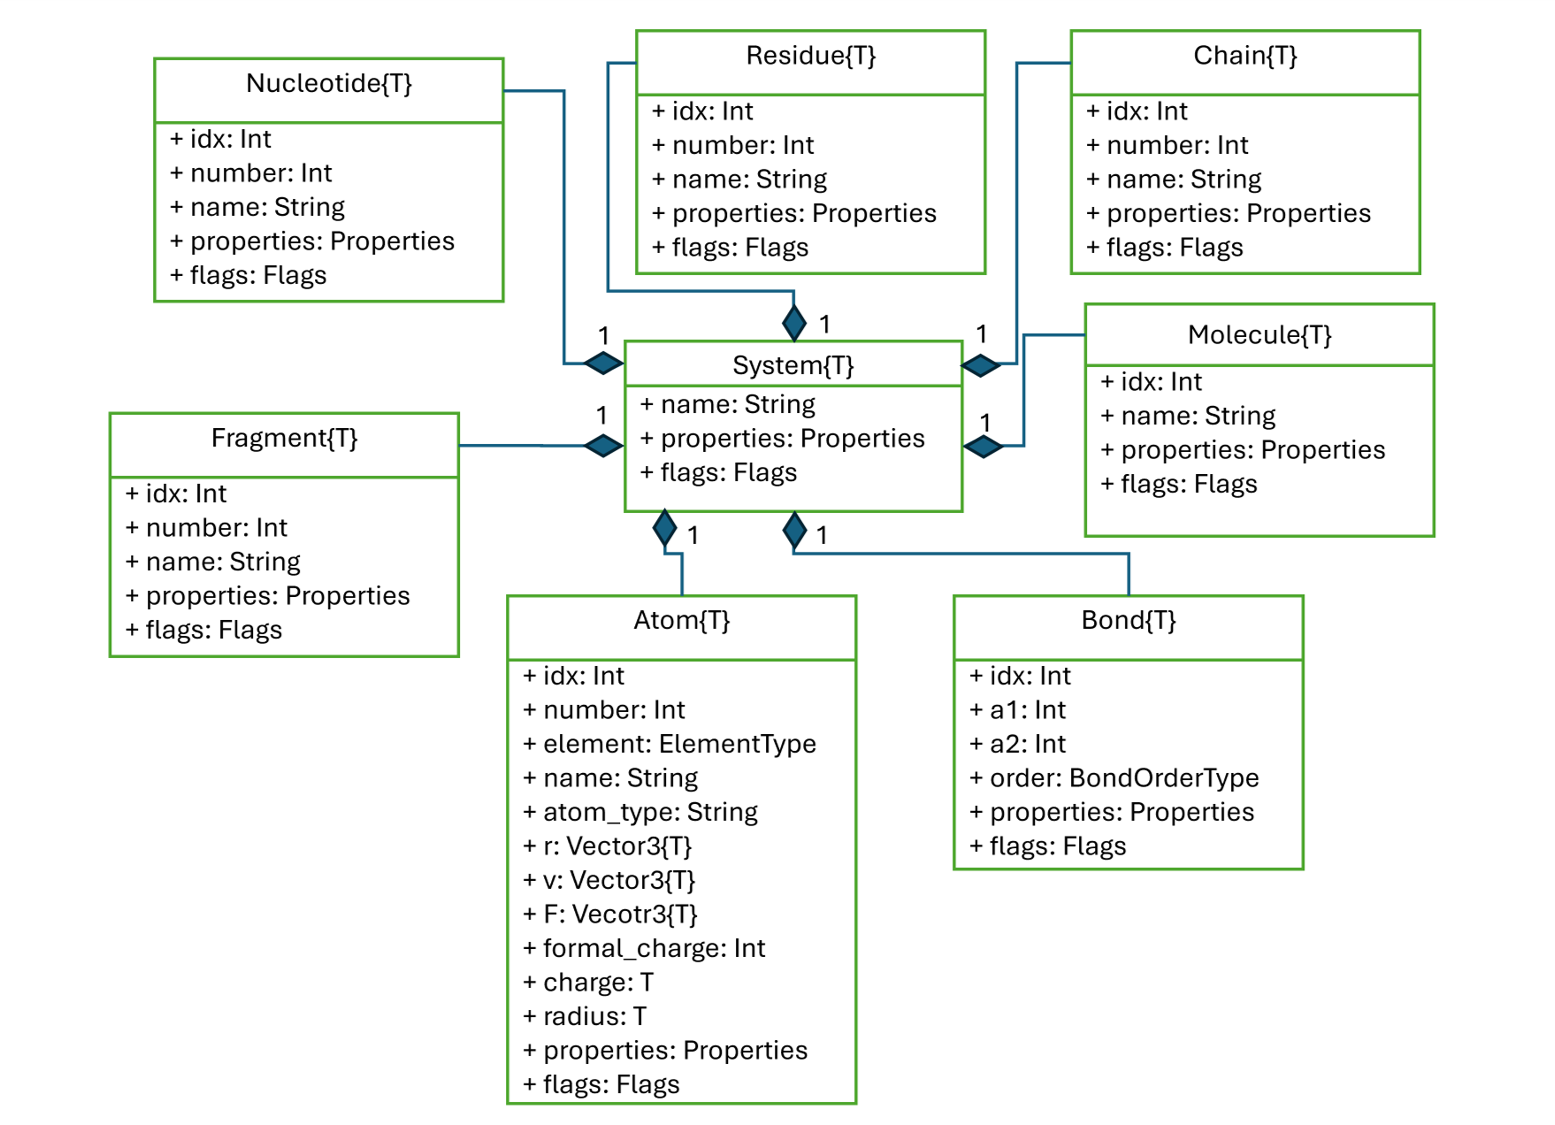
\includegraphics[width=15cm]{gfx/uml.png}}
	\caption{UML diagram of the core of \biochem. In the center resides the \texttt{System} interface. All other functionalities are grouped around that core piece. Only the most important functionalities of each class are  shown.}
	\label{fig:biochem_uml}
\end{figure*}



In this work we sought to redesign the popular \ball\ package for molecular analysis and simulation. This section examines reasons behind this redesign followed by descriptions detailing \biochem's core implementations.

\subsection{Reasons for a redesign: \textit{why Julia?}}

There remains an ongoing need in the structural bioinformatics ecosystem in Julia for a framework offering rich functionalities akin those provided by \ball.  While the design goals are still valid, their realization in \ball\ is not contemporary anymore. The choice regarding programming language impacts implementation of the mentioned design goals massively. From today's perspective in particular with regard to its purpose as a platform for RAD, the usage of C++ may be considered suboptimal. \\

As for many scientific software packages, the development times for applications play a crucial role for the acceptance and usability of the underlying library. For instance, significant time investment may often be required merely installing libraries alongside their dependencies. Despite using the CMake build system since version 1.3, setting up \ball\ remains a highly non-trivial task. \\
Moreover, knowledge surrounding utilized programming languages heavily influences development times. Low-level languages like C++ necessitate greater learning curves compared to scripting languages such as Python \cite{Ousterhout1998}. 
Even with the additional Python bindings, the integration of new functionality is still not straightforward. In contrast, the implementation of new features is typically associated with the addition of massive amounts of boilerplate code. This applies to an even greater extent in cases where portability to different platforms and compiler settings have to be supported. \\
Consequently, \ball\ itself can be considered as a textbook example for the two language problem. In the latter, the core functionality is often implemented in a low-level programming language, ensuring performance, whereas higher-level programming languages facilitate user-friendly interfaces towards the core functionalities \cite{Julia_what}. Julia was explicitly developed addressing these challenges \cite{Julia_accomplish}.\\ 
Nevertheless, it is important to keep in mind that back in 1996 and still in 2010, C++ was the best choice for the implementation ensuring performance required specifically within the contexts involving molecular mechanics applications. \\
Switching our development from C++ to Julia has greatly simplified conforming the design goals: 
\begin{itemize}
	\item Ease of use: \biochem's source code provides a better readability as the boilerplate code is massively reduced compared to \ball\ and the usage of C++. The integration of documentation, basic tutorials, and test cases facilitates the introduction to \biochem, not to mention the trivial installation via Julia's package manager. 
	
	\item Openness: Just like installations, the integration process surrounding external tools to \biochem\ is straightforward. Our well-documented interfaces allow nearly seamless integration of custom applications. 
	
	\item Robustness: One of the strengths of Julia is the integrated unit testing functionality allowing to test implemented code on the fly. \biochem\ has been carefully developed with accompanying test cases for the core structures as well as for the functionalities ensuring non-faulty behavior using \texttt{TestItemRunner.jl}\cite{TestItemRunner}. Benchmark test cases are implemented in order to assess performance of typical tasks with the help of \texttt{BenchmarkTools.jl} and \texttt{Pkgbenchmark.jl} \cite{BenchmarkTools.jl-2016, PkgBenchmark}. 
	
	\item Functionality: \biochem\ implements standard data structures for molecular entities and already provides different functionalities. These includes import of structures stored in common molecular data formats including PDB, PDBx/mmCIF, HyperChem HIN, SDF (Structured Data File), and PubChem JSON files. Molecular mechanics are offered through an interface for force fields and a concrete implementation for an AMBER force field. \biochem\ provides algorithms for structure minimization and structure mappings. The interfaces are designed in a way that facilitates adoption, e.g., the implementation of custom force fields or changing an optimizer for the structure minimization. 
\end{itemize}


\subsection{The core representation}

The core representation in \biochem\ centers around the \texttt{System} data structure, which serves as the foundation for all applications within the framework. As shown in Figure~\ref{fig:biochem_uml}, the system contains data structures for the representation of atoms, bonds, molecules, chains, residues, nucleotides, and fragments. These components are either generated explicitly or populated by reading input files (see code listing ~\ref{lst:rmsd-and-amber}). \\

The atom representation with its position, velocity, and force contributes substantially to the framework's efficiency. After initially considering \textit{DataFrames.jl} \cite{Bouchet-Valat2023}, we opted for a custom implementation of the \textit{Tables.jl} interface \cite{BouchetValat2018}. The custom implementation enabled greater flexibility regarding the interface design and improved performance in initial benchmarks.\\
The custom implementation maintains compatibility with DataFrames.jl through the shared Tables.jl interface, allowing straightforward conversion when needed. Additionally, support for conversion to \textit{AtomsBase.jl} representation is under development. Table~\ref{table2_benchmark_amber} presents a performance comparison between \ball\ and \biochem\ for processing an input structure with 892 atoms. 

\biochem\ is on par with its C++ predecessor in most tasks, with some operations like \texttt{compute\_forces} being slower. It is important to keep in mind, that several years of development have led to a highly optimized code base in \ball, while our implementation still undergoes improvements.
 
\begin{table}
	\tbl{Comparison of time requirements of the Amber force field implementations. The input file consisted of 892 atoms and was processed on the same system (AMP EPYC 7713 CPU, S/C/T=2/64/1).}{
		\begin{tabular}{|l|c|c|}\hline
			Description & \ball & \biochem  \\\hline
			\texttt{compute\_energy} & 3.89 ms & 4.706 ms \\
			\texttt{compute\_forces}	& 3.56 ms & 33.590 ms \\ 
			\texttt{update}	& 34.41 ms &  89.635 ms \\ 
			\texttt{setup}	& 72.04 ms & 70.604 ms \\ 
			\hline
	\end{tabular}}
	\label{table2_benchmark_amber}
\end{table}
 


